\documentclass[a4paper,10pt]{article}
\usepackage[utf8]{inputenc}
\usepackage{enumerate}
\usepackage{amsmath}
\usepackage{graphicx}
\usepackage{listings}
\usepackage{float}
\usepackage[caption = false]{subfig}
\usepackage[parfill]{parskip}
\usepackage{url}

\title{Project 1: model of a stellar core}
\author{Christer Dreierstad\footnote{I have been working together with Hans Erlend Bakken Glad.}}
\date{07.03.2018}

\begin{document}
\maketitle

%\section*{Abstract}
%The goal of this project is to create a model of the core of a star by solving %differential equations. Using values 



\section{Numerical model}
The numerical model consists of three parts. One part to find the total energy $\epsilon$, one for importing data consisting of temperature, radius and opacity and the main part of the model for solving the differential equations.

\subsection{Calculations of necessary variables}
By assumption hydrogen and helium are fully ionized, thus contributing with respectively one and two electrons. Since hydrogen contribute with one electron we have $n = 2\rho X/m_u$, where the factor 2 comes from the contribution of both the electron and the proton. Where $m_u$ is the unified atom mass unit, which for hydrogen is $1m_u$. For helium, with a mass unit of $4m_u$, $n = 3\rho Y/4m_u$. Metals contribute with the usual number of electrons resulting in $n = \rho Z /2m_u$. From this we have $n_{tot} = \rho/m_u(2X + 3Y/4 + Z/2)$ and the average molecular weight is given by $\mu = \rho/m_u n_{tot}$, which leads to 

\begin{align}\label{eq:mu}
\mu = \frac{1}{(2X + 3Y/4 + Z/2)},
\end{align} 

where X, Y and Z are the mass fractions. Since we are assuming the gas to be ideal, we can use the ideal gas law to calculate the gas pressure as we integrate. The number of particles in the gas can be expressed as $N = m/\mu m_u$. Inserting the aforementioned expression in the ideal gas we get $P = (m/\mu m_u)kT/V$, where we can insert the density $\rho = m/V$, yielding

\begin{align}\label{eq:pressure_gas}
P_{gas} = \frac{\rho}{\mu m_u} kT,
\end{align}

where k is Boltzmann's constant and T is the temperature. To calculate the full pressure we also need the radiation pressure $P_{rad} = aT^4/3$, where a is the radiation constant. This yields the final equation for pressure

\begin{align}\label{eq:pressure}
P = \frac{\rho}{\mu m_u} kT + \frac{a}{3}T^4.
\end{align}

Further we need an equation for the density, which we find from the solving equation \eqref{eq:pressure_gas} for $\rho$, giving us

\begin{align}\label{eq:density}
\rho = \frac{\mu m_u}{k T}P_{gas} = \frac{\mu m_u}{kT}(P - \frac{a}{3}T^4).
\end{align}

%\subsection{Calculating the energy $\epsilon$}



\subsection{Importing values and interpolating}
We have a grid of the opacity for given temperatures and radii, all given in logarithmic scale and in cgs units. To extract the values we do a 2 dimensional interpolation with a feature that comes with scipy. This feature extrapolates automatically. Since we are working with SI units, we have must convert g and cm to kg and m respectively. We construct a function that takes non-logarithmic arguments in SI units and converts them to logarithmic cgs. The function will take $\rho$ as an argument, and use the fact that the radii in the table are given as $R = \rho/(T\cdot10^{-6})^3$. The interpolation feature takes $\log_{10}(R)$ and $\log_{10}(T)$ in cgs as arguments and returns the opacity $\log_{10}(\kappa)$ in cgs, while the functions returns the opacity in SI.



\subsection{Solving the differential equations}
Using the Euler method to solve the differential equations, integrating inwards with small steps of the mass $dm$. Assuming that the gas is ideal we can further calculate the gas pressure along side the integration. We consider the integration as calculating the pressure, radius, temperature and luminosity shell by shell inwards from the bottom of the solar convection zone and to the center of the core. While integrating we also calculate the gas pressure and the mass m. Since we are using Eulers method the order of integrating the differential equations are not important, but we need to calculate the temperature $T_{i+1}$ and pressure $P_{i+1}$ in order to calculate the density $\rho_{i+1}$. Using Eulers method to integrate the differential equations are on the form

\begin{align}
r_{i+1} = r_i + \frac{dr_i}{dm}dm = r_i + \frac{1}{4\pi r_i^2 \rho_i}dm,
\end{align}

\begin{align}
P_{i+1} = P_i + \frac{dP_i}{dm}dm = P_i - \frac{Gm_i}{4\pi r_i^4}dm,
\end{align}

\begin{align}
L_{i+1} = L_i + \frac{dL_i}{dm}dm = L_i + \epsilon(T_i,\rho_i)dm,
\end{align}

\begin{align}
T_{i+1} = T_i + \frac{dT_i}{dm}dm = T_i - \frac{3\kappa(\rho_i,T_i)L_i}{256\pi^2 \sigma, r_i^4 T_i^4}dm
\end{align}

where G is the gravitational constant, $\epsilon(T_i,\rho_i)$ is the total energy, $\kappa(\rho_i,T_i)$ is the opacity discussed in the previous subsection and $\sigma$ is Stefan-Boltzmann's constant. Further we calculate the mass $m_{i+1} = m{i} + dm$, where dm must be negative since we are moving inwards to where the mass is zero. The density is calculated for each step by equation \eqref{eq:density}.


\subsection{Dynamic step length}
Implementing a dynamic step size allows the step size to vary as the data varies. If the change in the data are small, the step size will be larger than if the change in data are significant. This means that we will be performing less calculations over the parts of the data that are similar, while performing more calculations over the parts of that data that are of interest. The only modification we need to do in order to implement a dynamic step length is to calculate the new dm's. This is done by requiring that $|dr| < rp$ for a factor p that must be smaller than one. Solving the original differential equation for r with respect to dm we have $dm = dr/f$, where f is the function $dr/dm$, inserting the above requirement we get

\begin{align}
dm = \frac{dr}{f} = \frac{rp}{f}.
\end{align}

We now calculate a dm for each of the differential equations, to make sure we integrate properly we choose the smallest value of the dm's we calculated.

When choose a value for p, we start at 0.1 as suggested, and find that the mass rapidly falls towards zero. $p = 0.001$ resulted in the mass reaching after 243 steps, and the other differential equations were not calculated properly. A $p = 0.0001$ resulted in smooth plots.
 
%\begin{figure}[H]
%\centering
%\includegraphics[width=12cm]{}
%\caption{}
%\label{fig:}
%\end{figure}


\section{Experimenting with values}
\subsection{Initial conditions}
In the following subsection we will present the values (e.g. mass, density) as functions of radius, unless other is specified. The initial conditions were weighted by a factor five as per the boundaries of the project.
\begin{itemize}
\item Increasing $R_0$ both the mass and the luminosity falls further out in the core, meaning $r/R_0$ is close to 1. 

\item Decreasing $R_0$ yields the opposite of the last bullet; mass and luminosity falls closer to the center of the core.


\item Increasing $T_0$ the mass falls further out in the core. The luminosity falls faster the larger $T_0$'s.

\item Decreasing $T_0$ the luminosity falls further in the core. The larger the radius, the slower the decrease of the luminosity is. 

\item Increasing $\rho_0$ both the mass and the luminosity falls further out in the core. 

\item Decreasing $\rho_0$ yields the opposite of the last bullet; mass and luminosity falls closer to the center of the core.

\item A change in $P_0$ is equivalent to a change in $\rho_0$, as one would predict from the equation for pressure \eqref{eq:pressure}.
\end{itemize}

\subsection{Step length}
\begin{figure}[!]
\centering
\subfloat[Different values of dm in the same plot.]{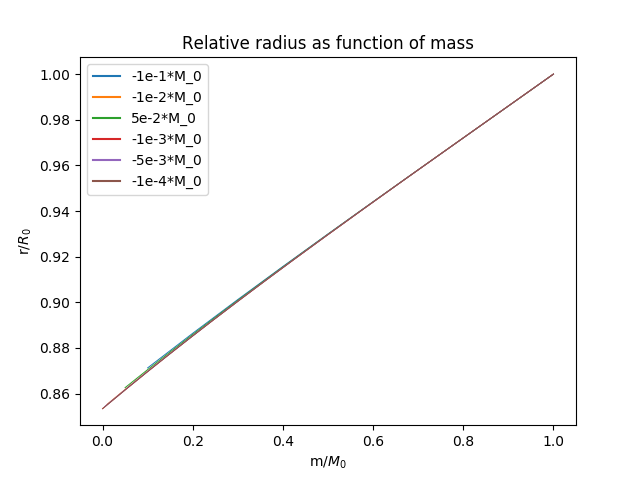
\includegraphics[width = 12cm]{dm_test.png}} \\
\subfloat[Zoom of the end part of (a).]{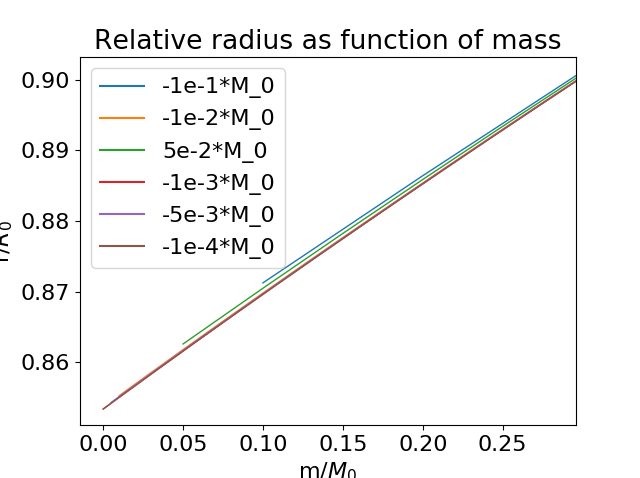
\includegraphics[width = 6cm]{dm_test_zoom_l.png}}
\subfloat[Zoom of the end part of (b).]{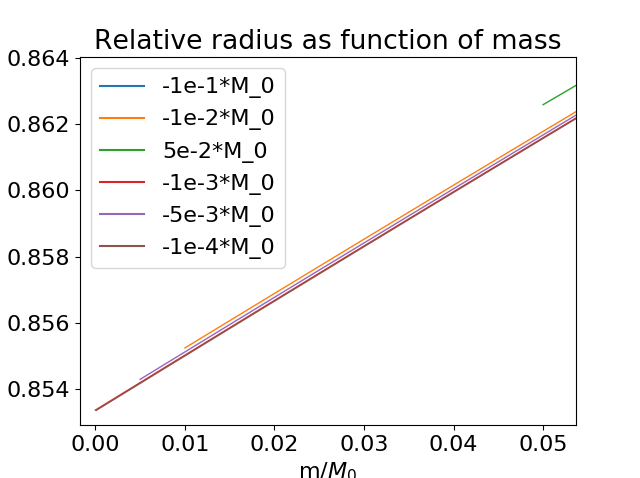
\includegraphics[width = 6cm]{dm_test_zoom_2_l.png}}
\caption{Relative radius as a function of the relative mass for different step length dm.}
\label{fig:dm_test}
\end{figure}

Changing the value of the step length dm we see in figure \ref{fig:dm_test} that we get the best results by using a smaller step length. By making the step size larger, the mass falls to zero faster. We can see in figure \ref{fig:dm_test} (b) that the plot of the largest dm 
results in the largest end values of both r and m. This is what one would expect since dm is proportional to dr by the differential equation $dr = (4\pi r^2 \rho)^{-1}dm$. A high resolution will neglect the finer details of the physics.



%PROBLEM: når økte rho_0 ble rho(r) rar, forklar.



%When varying the values of dm we  $-10^{-i}M_0$ where $-8 \leq i \leq -1$ where $i$ is an %integer.

\subsection{Creating a realistic model}
Starting out with tweaking the initial conditions of the luminosity, radius and temperature we want to make the mass and the radius fall towards zero, and afterwards tweak them further so that the luminosity falls to zero. The first model that was found had a higher density of $\approx1.6\rho_0$, lower temperature of $0.4T_0$ and lower radius $\approx 0.48R_0$. This model had the mass go to zero, while both the luminosity and the radius were close to zero, all well within the $\pm 5\%$ limit. The problem with the model, as one can see in figure \ref{fig:final_error}, is that the model proved unphysical at the center of the core, (specifically pressure and density), as well as on the edge of the core (specifically temperature and density). The problem regarding the behavior if tge density at the edge of the core was found to be the reduction of the initial temperature, which proved unphysical below $0.81T_0$. A lot of time was sadly spent on this model trying to modify it. 

Starting over, again with the goal of making the mass go to zero, the behavior of changing initial conditions were further (properly, one might say) studied. Referring to figure \ref{fig:testing_values} b, d and e, we found starting with $0.7R_0$, $0.5\rho$ and the original $T_0$ to be a good starting set of initial conditions. The best model was found to have $0.543R_0$, $1.5T_0$ and $0.63\rho_0$. The end result was a mass of $m/M_0 \approx 0.023$, $r/R_0 \approx 0.025$ and $L/L_0 \approx 0.0008$.


%\begin{figure}[!]
%\centering
%\subfloat[]{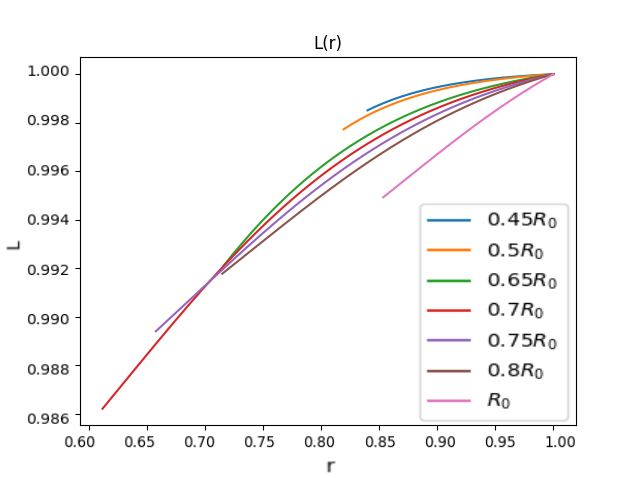
\includegraphics[width = 6cm]{R_0_tests_2_L(r).png}} 
%\subfloat[]{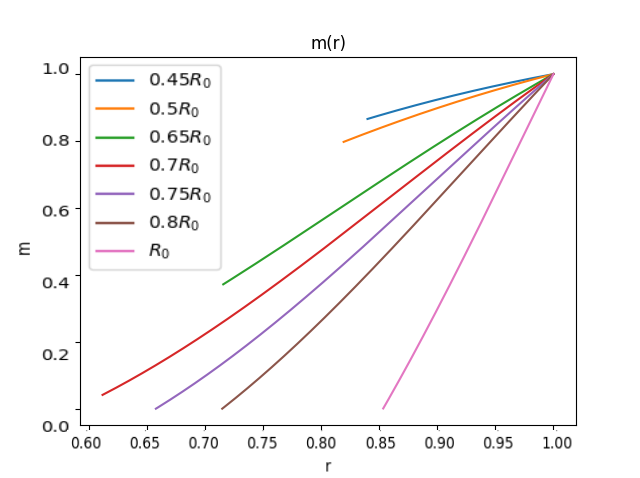
\includegraphics[width = 6cm]{R_0_tests_2_m(r).png}} \\
%\subfloat[]{\includegraphics[width = 6cm]{} 
%\subfloat[]{\includegraphics[width = 6cm]{}} \\
%\subfloat[]{\includegraphics[width = 6cm]{}} 
%\subfloat[]{\includegraphics[width = 6cm]{}}
%\caption{TEKSTKETKETKETK}
%\label{fig:dm_test}
%\end{figure}

\begin{figure}[!]
\centering
\subfloat[]{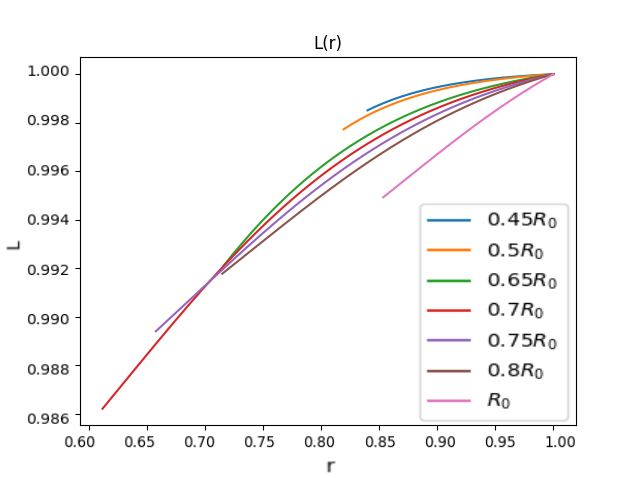
\includegraphics[width = 6cm]{R_0_tests_2_L(r).png}} 
\subfloat[]{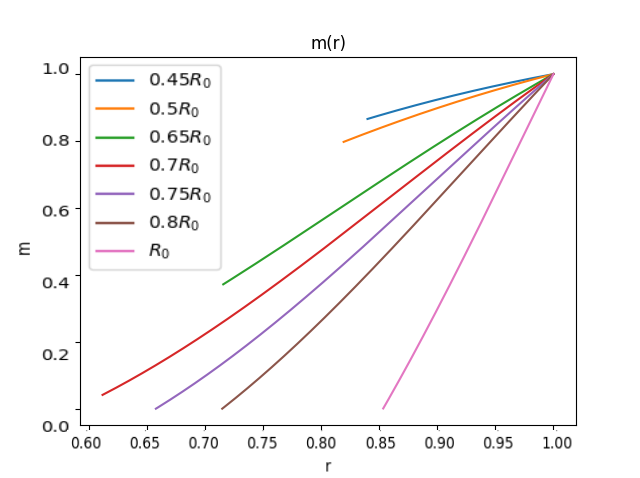
\includegraphics[width = 6cm]{R_0_tests_2_m(r).png}} \\
\subfloat[]{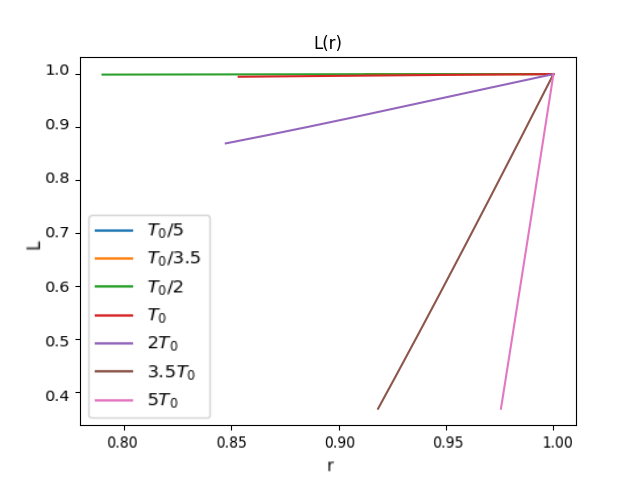
\includegraphics[width = 6cm]{T_0_tests_L(r).png}} 
\subfloat[]{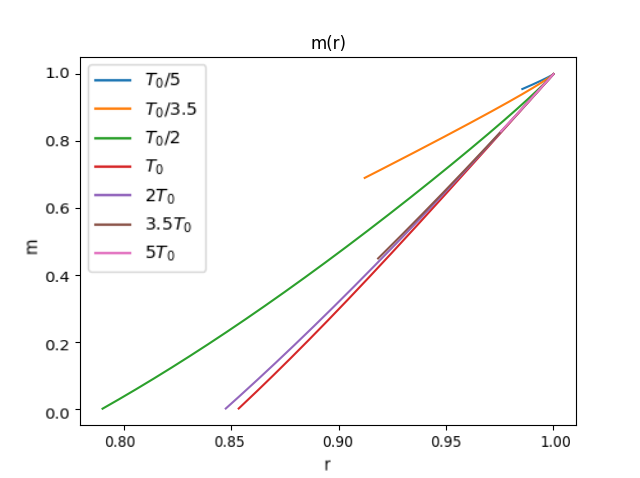
\includegraphics[width = 6cm]{T_0_tests_m(r).png}} \\
\subfloat[]{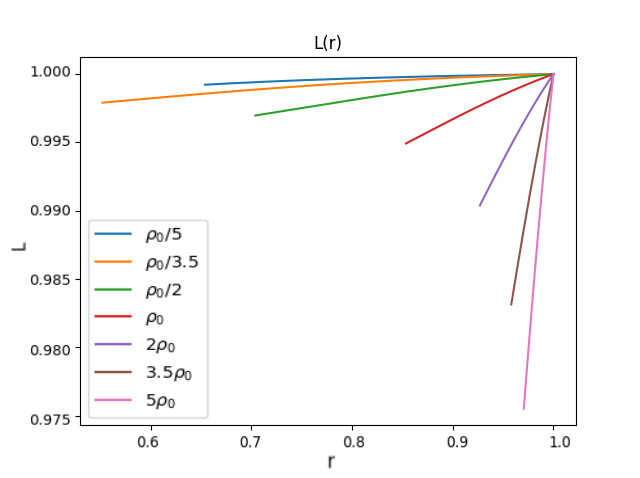
\includegraphics[width = 6cm]{rho_0_tests_L(r).png}} 
\subfloat[]{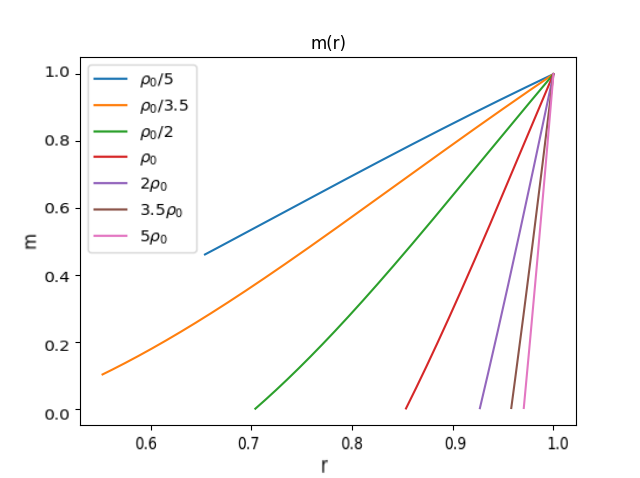
\includegraphics[width = 6cm]{rho_0_tests_m(r).png}}
\caption{Different initial conditions for the temperature, density and radius. The left (a, c and e) three plots are of the luminosity, while the right (b, d and f) are of the mass, both as functions of the radius.}
\label{fig:testing_values}
\end{figure}




\begin{figure}[!]
\centering
\subfloat[]{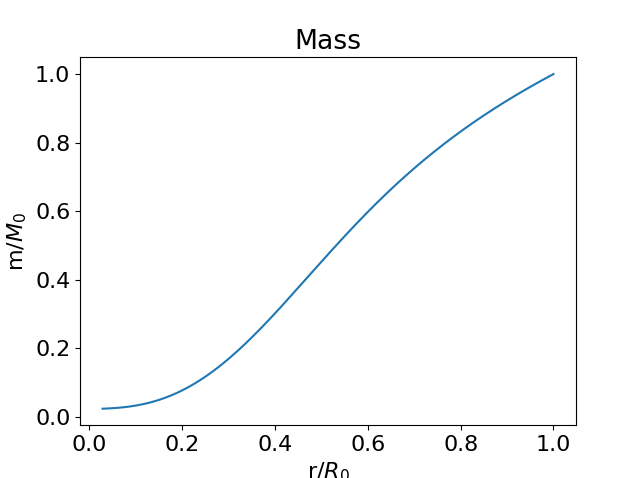
\includegraphics[width = 6cm]{m(r)_l.png}} 
\subfloat[Logarithmic scale of $P/P_0$.]{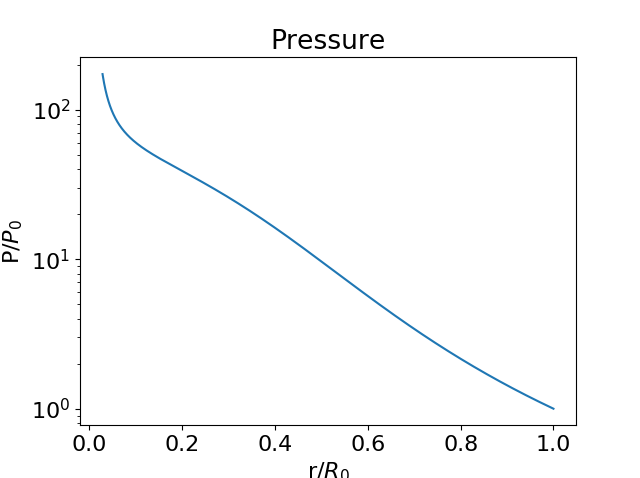
\includegraphics[width = 6cm]{P(r)_l.png}} \\
\subfloat[Logarithmic scale of $\rho/\rho_0$.]{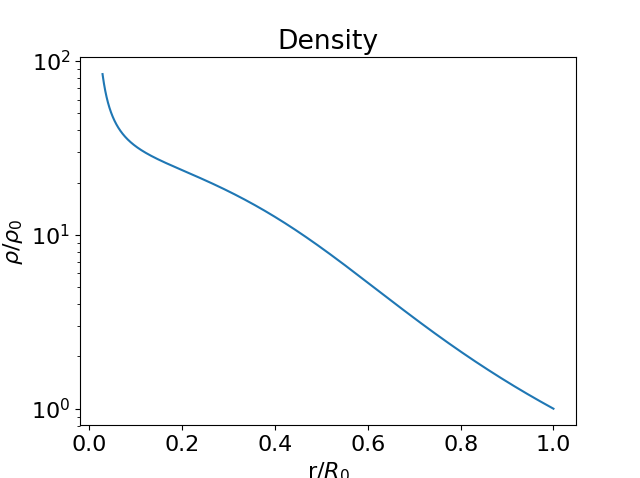
\includegraphics[width = 6cm]{rho(r)_l.png}} 
\subfloat[Logarithmic scale of $\epsilon/\epsilon_0$.]{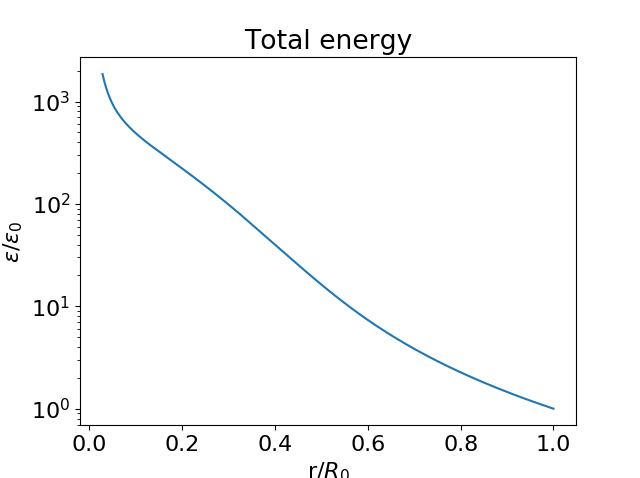
\includegraphics[width = 6cm]{eps(r).png}} \\
\subfloat[]{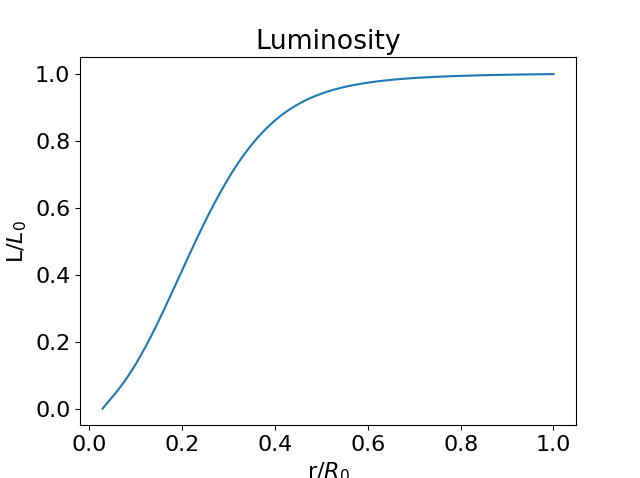
\includegraphics[width = 6cm]{L(r)_l.png}} 
\subfloat[]{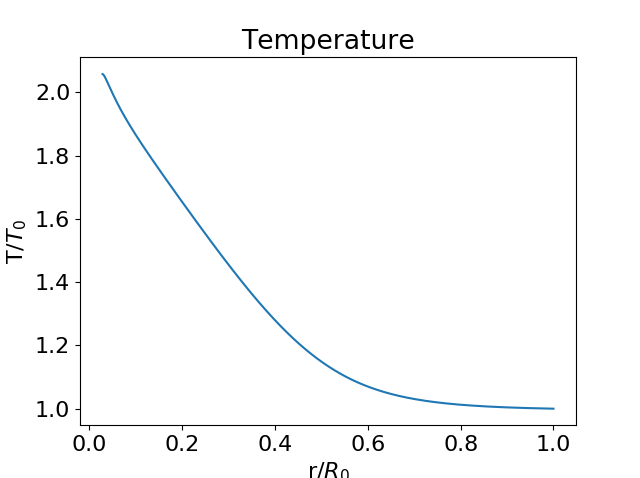
\includegraphics[width = 6cm]{T(r)_l.png}}
\caption{Respective relative values as a function of relative radius. The plots are based on the best model that was found for the initial conditions of the radius, temperature and density.}
\label{fig:final}
\end{figure}

\begin{figure}[!]
\centering
\subfloat[]{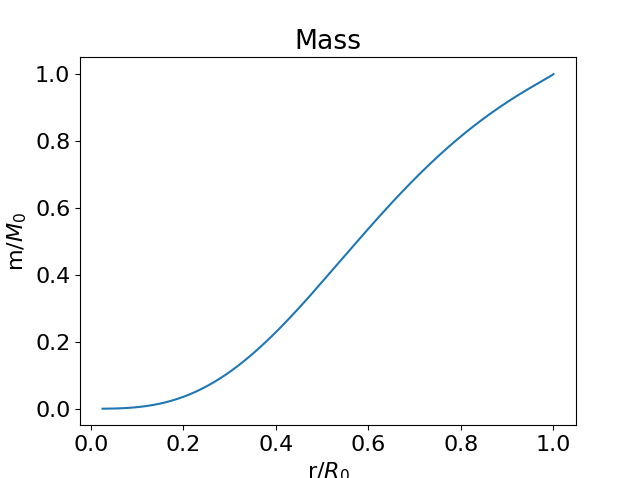
\includegraphics[width = 6cm]{m(r)_feil.png}} 
\subfloat[]{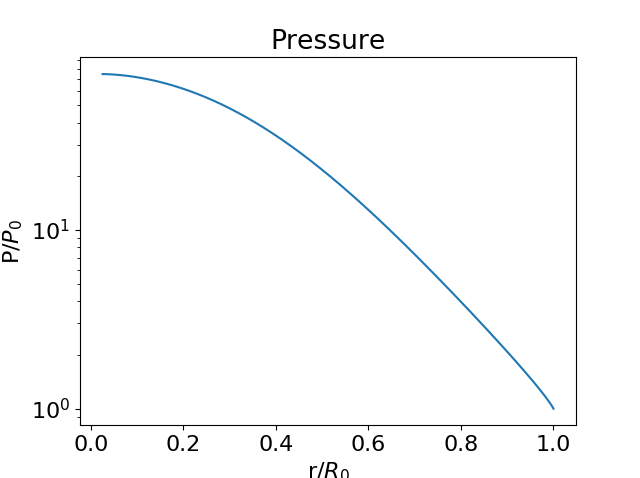
\includegraphics[width = 6cm]{P(r)_feil.png}} \\
\subfloat[]{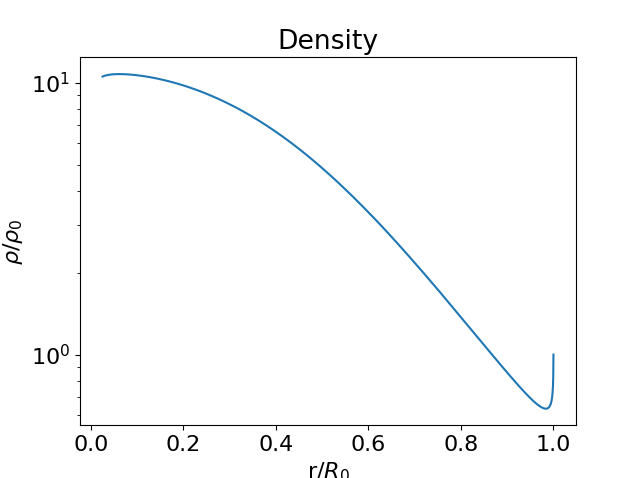
\includegraphics[width = 6cm]{rho(r)_feil.png}} 
\subfloat[]{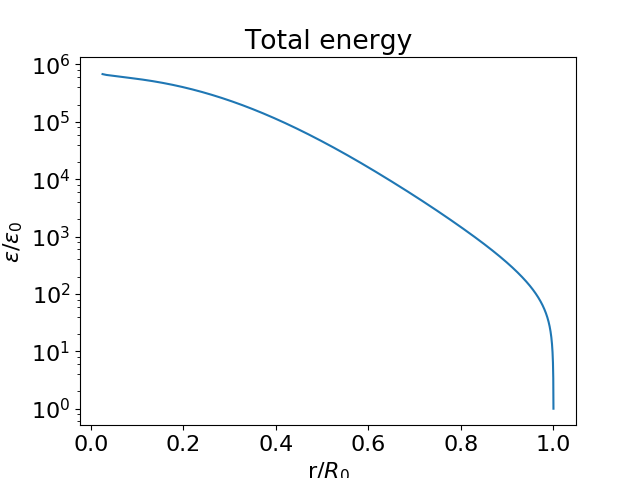
\includegraphics[width = 6cm]{eps(r)_feil.png}} \\
\subfloat[]{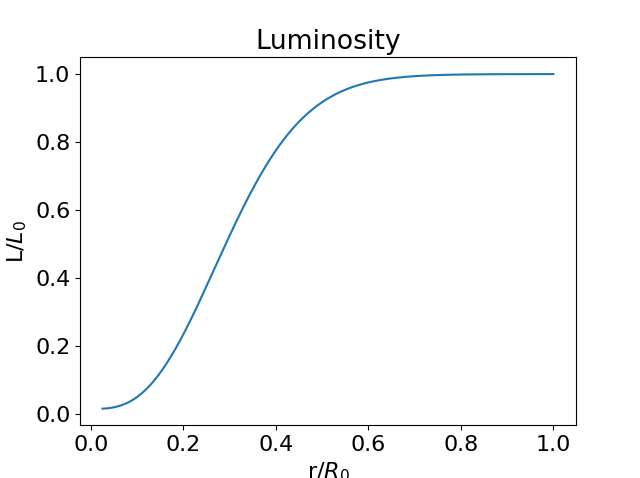
\includegraphics[width = 6cm]{L(r)_feil.png}} 
\subfloat[]{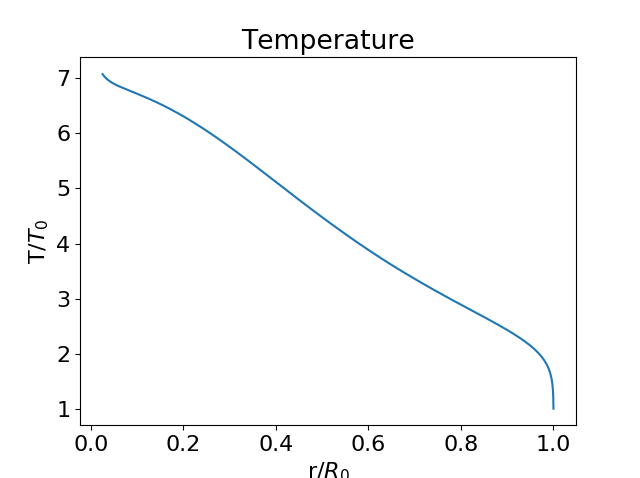
\includegraphics[width = 6cm]{T(r)_feil.png}}
\caption{The failed initial condition modification. Respective relative values as a function of relative radius.}
\label{fig:final_error}
\end{figure}


\begin{thebibliography}{9}

\bibitem{lamport94}
  B. V. Gudiksen,
  \textit{Variable Steplength},
  \url{http://www.uio.no/studier/emner/matnat/astro/AST3310/v18/beskjeder/variablesteplength.pdf} (downloaded 07.03.18)

\bibitem{2}
  B. V. Gudiksen,
  \textit{AST3310: Astrophysical plasma and stellar interiors},
  \url{http://www.uio.no/studier/emner/matnat/astro/AST3310/v18/beskjeder/notes_v1.pdf} (downloaded 07.03.18)
\end{thebibliography}






\end{document}